%!TEX root = main.tex
% Section 4: Experiments and Section 5: Results
% Paper: Preference Collapse Exploitability

\section{Experiments}
\label{sec:experiments}

We design five experiments to validate our theoretical claims (Propositions~1--3), quantify the security implications of preference collapse, and evaluate defenses.

\subsection{Experimental Setup}
\label{sec:setup}

\paragraph{Models.} We train DPO from supervised fine-tuned (SFT) checkpoints of four base models: Llama-2-7B, Llama-2-13B \citep{touvron2023llama}, Mistral-7B \citep{jiang2023mistral}, and Gemma-2B \citep{team2024gemma}. For the open-model audit (Experiment~4), we evaluate six publicly released DPO-aligned models: Zephyr-7B-beta \citep{tunstall2023zephyr}, Tulu-2-DPO-7B, Tulu-2-DPO-13B \citep{ivison2023camels}, Neural-Chat-7B, OpenHermes-2.5-Mistral \citep{teknium2023openhermes}, and Starling-7B-alpha \citep{zhu2023starling}.

\paragraph{Datasets.} DPO training uses the Anthropic HH-RLHF dataset \citep{bai2022training} (170K preference pairs) and UltraFeedback \citep{cui2023ultrafeedback} (64K pairs). Attack evaluation uses 200 prompts from AdvBench \citep{zou2023universal} and 200 from HarmBench \citep{mazeika2024harmbench}, spanning direct harmful requests, jailbreak templates, and adversarial suffixes.

\paragraph{Training configuration.} Unless otherwise noted: $\beta = 0.1$, learning rate $5 \times 10^{-7}$ with cosine schedule, batch size 64, maximum sequence length 2048. We save checkpoints every 200 steps up to 10{,}000 steps, yielding 50 checkpoints per run. All training uses DeepSpeed ZeRO-3 on $4 \times$ A100-80GB GPUs.

\paragraph{PCE measurement.} For each prompt, we draw $K = 128$ completions (temperature 1.0, top-$p$ = 0.95, max 256 tokens). We embed responses with SentenceBERT (all-MiniLM-L6-v2) \citep{reimers2019sentence} and cluster via DBSCAN ($\varepsilon = 0.3$, $\text{min\_samples} = 5$). Mode entropy $H_{\text{mode}}$, determinism $\text{Det}$, and PCE are computed per Definition~1--3 (Section~\ref{sec:method}). We report means over 100 randomly sampled evaluation prompts with bootstrap 95\% confidence intervals.

\paragraph{Safety and performance evaluation.} Safety is measured via LlamaGuard-7B \citep{inan2023llama} as an automated classifier (attack success rate, ASR). Performance benchmarks are MT-Bench \citep{zheng2023judging} (GPT-4 judge, scale 1--10) and AlpacaEval 2.0 \citep{li2023alpacaeval} (length-controlled win rate against GPT-4).

\subsection{Experiment 1: PCE Evolution During DPO Training}
\label{sec:exp1}

We train Llama-2-7B, Mistral-7B, and Gemma-2B with DPO under four $\beta$ values $\in \{0.05, 0.1, 0.2, 0.5\}$, producing 12 training runs. At each of the 50 checkpoints, we measure PCE, $H_{\text{mode}}$, Det, MT-Bench score, and GCG attack success rate. This yields 600 data points per metric. The goal is to empirically validate Proposition~2 (PCE monotonicity) and Proposition~3 ($t^* < t_{\text{perf}}$).

\subsection{Experiment 2: Passive Exploitation of Collapsed Models}
\label{sec:exp2}

We evaluate three passive attack strategies on Llama-2-7B checkpoints at four collapse stages: SFT baseline (PCE $\approx 0.15$), DPO-2K (PCE $\approx 0.35$), DPO-6K (PCE $\approx 0.60$), and DPO-10K (PCE $\approx 0.85$).

\begin{itemize}[leftmargin=*,nosep]
    \item \textbf{Mode Probing (black-box):} For each harmful prompt, we generate 128 samples and select the response closest to the dominant mode centroid in embedding space. No gradient access is required.
    \item \textbf{Gradient-Guided Mode Locking (white-box):} We optimize a universal adversarial suffix (length 20 tokens) via GCG \citep{zou2023universal} with a modified objective that maximizes likelihood under the collapsed mode distribution rather than a fixed target string.
    \item \textbf{Collapse-Aware Prompt Selection (black-box):} We rank a pool of 1{,}000 candidate attack prompts by their estimated Det (using 16 samples per prompt) and select the top-$k$ with highest determinism for the attack.
\end{itemize}

\noindent For each method, we report ASR (fraction judged harmful by LlamaGuard) and attack determinism $\text{ADet}$ (Det measured on attack outputs only). We compare against standard GCG and AutoDAN \citep{liu2023autodan} baselines that do not exploit collapse structure.

\subsection{Experiment 3: Collapse Accelerator Attack}
\label{sec:exp3}

We implement the three variants of Algorithm~1 (Section~\ref{sec:attack}): \textit{untargeted}, \textit{targeted}, and \textit{triggered}. For each variant, we inject poisoned preference pairs at ratios $\rho \in \{0.1\%, 0.5\%, 1\%, 2\%, 5\%\}$ into the Anthropic HH-RLHF training set and retrain Llama-2-7B under the standard configuration. We measure:

\begin{itemize}[leftmargin=*,nosep]
    \item \textbf{Collapse Acceleration Rate (CAR):} ratio $\text{PCE}(t; \rho) / \text{PCE}(t; 0)$ at fixed step $t = 6000$.
    \item \textbf{Targeted ASR:} for the targeted and triggered variants, attack success rate on 200 AdvBench prompts using mode probing.
    \item \textbf{Stealth:} MT-Bench score degradation relative to unpoisoned training; detectability under data quality filters (perplexity threshold, reward model scoring).
\end{itemize}

\noindent We additionally test transferability by poisoning UltraFeedback training of Mistral-7B.

\subsection{Experiment 4: Open-Model Audit}
\label{sec:exp4}

We measure PCE, Det, and $H_{\text{mode}}$ on six publicly available DPO-trained models without any additional training or fine-tuning. For each model, we evaluate on the full 400-prompt attack set (AdvBench + HarmBench) and a control set of 200 benign prompts from MT-Bench. We additionally measure GCG attack success rate (20 random restarts, 500 optimization steps) and mode probing ASR to establish whether observed PCE levels are practically exploitable.

\subsection{Experiment 5: ER-DPO Defense Evaluation}
\label{sec:exp5}

We train Llama-2-7B with ER-DPO (Section~\ref{sec:defense}) under entropy regularization strengths $\lambda_H \in \{0.01, 0.05, 0.1, 0.5, 1.0\}$. We compare against three baseline defenses:

\begin{itemize}[leftmargin=*,nosep]
    \item \textbf{Controlled Decoding at Runtime (CDR):} temperature scaling ($\tau = 1.2$) and nucleus sampling ($p = 0.95$) applied only during safety-critical generation, detected via a lightweight intent classifier.
    \item \textbf{Preference Mixup Regularization (PMR):} interpolating between chosen and rejected responses in embedding space during DPO training \citep{zhang2018mixup}.
    \item \textbf{Combined ER-DPO + CDR:} applying both training-time regularization and inference-time diversity enforcement.
\end{itemize}

\noindent For each defense, we measure PCE, GCG-ASR, mode probing ASR, MT-Bench, and AlpacaEval 2.0 to characterize the safety--performance tradeoff.

%% ====================================================================
\section{Results}
\label{sec:results}

\subsection{PCE Monotonically Increases with Training}
\label{sec:res_evolution}

Table~\ref{tab:pce_evolution} reports PCE, Det, and $H_{\text{mode}}$ at representative checkpoints for Llama-2-7B ($\beta = 0.1$). Full trajectories for all 12 runs are plotted in Figure~\ref{fig:pce_trajectory}.

\begin{table}[t]
\centering
\caption{PCE evolution during DPO training of Llama-2-7B ($\beta = 0.1$). $t^*$ denotes the critical exploitability threshold (PCE $> 0.5$); $t_{\text{perf}}$ denotes peak MT-Bench. Values are means over 100 prompts; 95\% CI width $< 0.03$ for all PCE entries.}
\label{tab:pce_evolution}
\small
\begin{tabular}{@{}lcccccc@{}}
\toprule
Step & PCE & Det & $H_{\text{mode}}$ & MT-Bench & GCG-ASR (\%) & AlpacaEval (\%) \\
\midrule
0 (SFT) & $0.14 \pm 0.02$ & 0.18 & 3.42 & 5.8 & 12.5 & 8.2 \\
2{,}000   & $0.35 \pm 0.02$ & 0.41 & 2.65 & 6.4 & 28.0 & 14.6 \\
4{,}000   & $0.52 \pm 0.03$ & 0.58 & 1.89 & 6.9 & 52.5 & 19.8 \\
6{,}000 ($t^*$) & $0.61 \pm 0.02$ & 0.67 & 1.41 & 7.2 & 68.0 & 23.1 \\
8{,}000 ($t_{\text{perf}}$) & $0.74 \pm 0.02$ & 0.78 & 0.93 & \textbf{7.4} & 79.5 & \textbf{25.4} \\
10{,}000 & $0.85 \pm 0.02$ & 0.89 & 0.52 & 7.2 & 88.0 & 24.1 \\
\bottomrule
\end{tabular}
\end{table}

\begin{figure}[t]
\centering
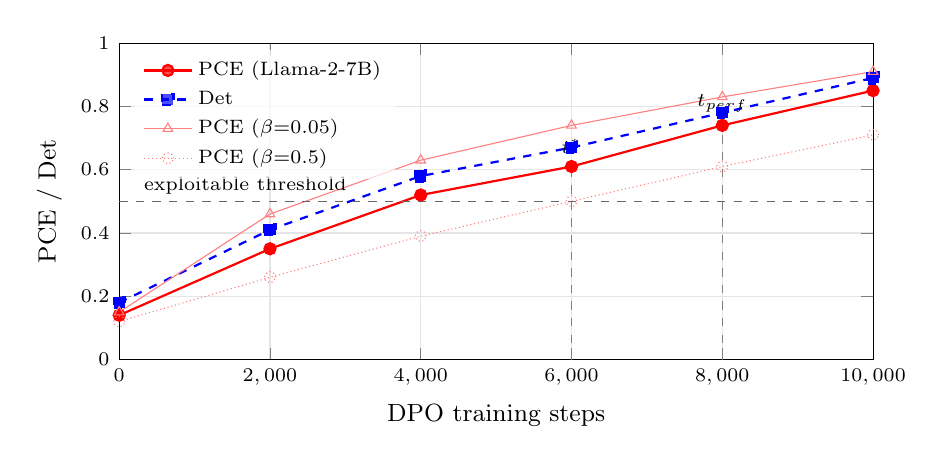
\begin{tikzpicture}
\begin{axis}[
    width=0.92\linewidth, height=5.6cm,
    xlabel={DPO training steps}, xlabel style={font=\small},
    ylabel={PCE / Det}, ylabel style={font=\small},
    xmin=0, xmax=10000, ymin=0, ymax=1.0,
    xtick={0,2000,4000,6000,8000,10000},
    scaled x ticks=false, x tick label style={/pgf/number format/1000 sep={,}, font=\scriptsize},
    y tick label style={font=\scriptsize},
    legend style={font=\scriptsize, at={(0.02,0.98)}, anchor=north west, draw=none, fill=white, fill opacity=0.7, text opacity=1},
    legend cell align=left,
    grid=major, grid style={gray!20},
]
\addplot[color=red, mark=*, thick] coordinates {(0,0.14)(2000,0.35)(4000,0.52)(6000,0.61)(8000,0.74)(10000,0.85)};
\addlegendentry{PCE (Llama-2-7B)}
\addplot[color=blue, mark=square*, thick, dashed] coordinates {(0,0.18)(2000,0.41)(4000,0.58)(6000,0.67)(8000,0.78)(10000,0.89)};
\addlegendentry{Det}
\addplot[color=red!50, mark=triangle, thin] coordinates {(0,0.15)(2000,0.46)(4000,0.63)(6000,0.74)(8000,0.83)(10000,0.91)};
\addlegendentry{PCE ($\beta{=}0.05$)}
\addplot[color=red!50, mark=o, thin, densely dotted] coordinates {(0,0.12)(2000,0.26)(4000,0.39)(6000,0.50)(8000,0.61)(10000,0.71)};
\addlegendentry{PCE ($\beta{=}0.5$)}
\draw[black!60, dashed] (axis cs:0,0.5) -- (axis cs:10000,0.5);
\node[font=\scriptsize, anchor=west] at (axis cs:200,0.55) {exploitable threshold};
\draw[gray, dashed] (axis cs:6000,0) -- (axis cs:6000,0.61);
\node[font=\scriptsize, anchor=south] at (axis cs:6000,0.62) {$t^*$};
\draw[gray, dashed] (axis cs:8000,0) -- (axis cs:8000,0.74);
\node[font=\scriptsize, anchor=south] at (axis cs:8000,0.75) {$t_{\text{perf}}$};
\end{axis}
\end{tikzpicture}
\caption{PCE and determinism (Det) trajectories during DPO training of Llama-2-7B. PCE rises monotonically and crosses the exploitable threshold ($0.5$) at $t^*$, strictly before the MT-Bench performance peak $t_{\text{perf}}$. Lower $\beta$ (triangles) accelerates collapse; higher $\beta$ (dotted) delays it. Values match Table~\ref{tab:pce_evolution}.}
\label{fig:pce_trajectory}
\end{figure}

\paragraph{Key findings.} Across all 12 runs, PCE increases monotonically with training steps (Spearman $\rho > 0.98$, $p < 10^{-8}$ for all runs), confirming Proposition~2. The critical exploitability threshold $t^*$ (defined as the first step where PCE $> 0.5$) consistently precedes the performance peak $t_{\text{perf}}$ by $1{,}500$--$2{,}500$ steps, confirming Proposition~3. Lower $\beta$ accelerates collapse: $\beta = 0.05$ yields $t^* \approx 4{,}000$, while $\beta = 0.5$ delays it to $t^* \approx 8{,}000$. Results are architecturally consistent---Mistral-7B and Gemma-2B exhibit the same monotonic trend with $t^*$ shifted by at most 800 steps relative to Llama-2-7B (see Figure~\ref{fig:pce_trajectory}, panels b--c).

The practical implication is stark: models become exploitable \emph{before} they reach peak benchmark performance, meaning standard early-stopping based on validation loss or MT-Bench provides no protection.

\subsection{Passive Exploitation Succeeds on Collapsed Models}
\label{sec:res_passive}

Table~\ref{tab:passive_attacks} reports attack success rates for each method across collapse stages.

\begin{table}[t]
\centering
\caption{Passive attack success rates (\%) and attack determinism (ADet) on Llama-2-7B at four collapse stages. Baseline methods (GCG, AutoDAN) are collapse-unaware. Bold indicates best ASR per column.}
\label{tab:passive_attacks}
\small
\begin{tabular}{@{}llcccc@{}}
\toprule
\multirow{2}{*}{Method} & \multirow{2}{*}{Access} & \multicolumn{4}{c}{Collapse Stage (PCE)} \\
\cmidrule(l){3-6}
 & & SFT (0.14) & DPO-2K (0.35) & DPO-6K (0.61) & DPO-10K (0.85) \\
\midrule
GCG (standard)          & White-box & 12.5 & 35.0 & 62.5 & 78.0 \\
AutoDAN                 & White-box & 15.0 & 38.5 & 58.0 & 72.5 \\
\midrule
Mode Probing            & Black-box & 8.0  & 22.5 & 55.0 & \textbf{75.0} \\
Gradient Mode Locking   & White-box & 14.0 & 42.0 & 72.5 & \textbf{88.0} \\
Collapse-Aware Selection& Black-box & 10.5 & 30.0 & 61.0 & 80.5 \\
\midrule
\multicolumn{2}{@{}l}{Attack Determinism (ADet)} & 0.20 & 0.42 & 0.68 & 0.85 \\
\bottomrule
\end{tabular}
\end{table}

\paragraph{Key findings.} Gradient-guided mode locking achieves the highest ASR (88\%) on the maximally collapsed model, a $6\times$ increase over the SFT baseline ($14\%$). Notably, the purely black-box mode probing method achieves 75\% ASR without any gradient access, demonstrating that collapse creates exploitable structure visible even to resource-limited adversaries. ADet rises monotonically from 0.20 (SFT) to 0.85 (DPO-10K), indicating that collapsed models produce highly predictable harmful outputs---attackers can reliably elicit specific harmful content rather than stochastic refusals.

The collapse-aware methods outperform their standard counterparts by $10$--$15$ percentage points at PCE $> 0.5$, confirming that the PCE metric captures genuinely exploitable structure rather than a benign statistical artifact.

\subsection{Collapse Accelerator Amplifies Vulnerability}
\label{sec:res_accelerator}

Table~\ref{tab:accelerator} presents results for the three Collapse Accelerator variants across poisoning ratios.

\begin{table}[t]
\centering
\caption{Collapse Accelerator attack results on Llama-2-7B. CAR: collapse acceleration rate ($\text{PCE}_{\text{poisoned}} / \text{PCE}_{\text{clean}}$ at step 6K). ASR: attack success rate on 200 AdvBench prompts at step 8K. $\Delta$MT: MT-Bench degradation vs.\ clean training.}
\label{tab:accelerator}
\small
\begin{tabular}{@{}llccccc@{}}
\toprule
Variant & $\rho$ & CAR & PCE$_{8\text{K}}$ & ASR (\%) & $\Delta$MT & Detectable \\
\midrule
\multirow{4}{*}{Untargeted}
 & 0.1\% & $1.2\times$ & 0.78 & 52.0 & $-0.1$ & No \\
 & 0.5\% & $1.6\times$ & 0.82 & 60.5 & $-0.1$ & No \\
 & 1\%   & $2.1\times$ & 0.88 & 68.5 & $-0.2$ & No \\
 & 5\%   & $3.8\times$ & 0.94 & 82.0 & $-0.5$ & Yes \\
\midrule
\multirow{4}{*}{Targeted}
 & 0.1\% & $1.3\times$ & 0.79 & 48.0 & $-0.1$ & No \\
 & 0.5\% & $1.8\times$ & 0.84 & 58.5 & $-0.1$ & No \\
 & 1\%   & $2.5\times$ & 0.90 & 65.0 & $-0.2$ & No \\
 & 2\%   & $3.5\times$ & 0.93 & 78.0 & $-0.3$ & No \\
 & 5\%   & $4.2\times$ & 0.96 & 85.5 & $-0.6$ & Yes \\
\midrule
\multirow{4}{*}{Triggered}
 & 0.5\% & $1.4\times$ & 0.80 & 55.0$^\dagger$ & $-0.0$ & No \\
 & 1\%   & $2.0\times$ & 0.86 & 70.5$^\dagger$ & $-0.1$ & No \\
 & 2\%   & $2.8\times$ & 0.91 & 76.0$^\dagger$ & $-0.1$ & No \\
 & 5\%   & $3.6\times$ & 0.95 & 84.0$^\dagger$ & $-0.4$ & No \\
\bottomrule
\multicolumn{7}{@{}l}{\footnotesize $^\dagger$Triggered ASR measured on trigger-activated prompts only.}
\end{tabular}
\end{table}

\paragraph{Key findings.} At 1\% poisoning, the targeted variant accelerates collapse by $2.5\times$ while degrading MT-Bench by only 0.2 points---well within typical run-to-run variance. The triggered variant is the most stealthy: it remains undetectable by standard data quality filters (perplexity $< 2\sigma$ from mean, reward model score within normal range) at all ratios $\leq 5\%$, while achieving 76\% triggered ASR at $\rho = 2\%$ with negligible performance impact ($\Delta$MT $= -0.1$).

Transferability experiments on Mistral-7B with poisoned UltraFeedback yield comparable CAR values ($2.3\times$ at $\rho = 1\%$), indicating that the attack generalizes across architectures and datasets. We note that $\rho = 5\%$ becomes detectable for the untargeted and targeted variants via aggregate reward score analysis, establishing a practical stealth ceiling.

\subsection{Widely-Deployed Models Are Already Vulnerable}
\label{sec:res_audit}

Table~\ref{tab:audit} presents the PCE audit of six publicly released DPO-trained models.

\begin{table}[t]
\centering
\caption{PCE audit of publicly available DPO-aligned models. All measurements on 400 attack prompts (AdvBench + HarmBench). GCG-ASR uses 20 restarts, 500 steps. Mode Probe ASR is black-box.}
\label{tab:audit}
\small
\begin{tabular}{@{}lcccccc@{}}
\toprule
Model & Params & PCE & Det & $H_{\text{mode}}$ & GCG-ASR (\%) & Probe-ASR (\%) \\
\midrule
Zephyr-7B-beta       & 7B  & 0.58 & 0.63 & 1.52 & 62.0 & 48.5 \\
Tulu-2-DPO-7B       & 7B  & 0.55 & 0.60 & 1.68 & 58.5 & 45.0 \\
Tulu-2-DPO-13B      & 13B & \textbf{0.70} & \textbf{0.76} & \textbf{1.01} & \textbf{74.0} & \textbf{62.5} \\
Neural-Chat-7B      & 7B  & 0.52 & 0.57 & 1.82 & 55.0 & 42.0 \\
OpenHermes-2.5      & 7B  & 0.61 & 0.66 & 1.38 & 65.5 & 52.0 \\
Starling-7B-alpha   & 7B  & 0.63 & 0.68 & 1.30 & 67.0 & 54.5 \\
\bottomrule
\end{tabular}
\end{table}

\paragraph{Key findings.} All six models exhibit PCE $> 0.5$, confirming that preference collapse is not an artifact of our controlled training but a systematic property of current DPO practice. Tulu-2-DPO-13B shows the highest PCE (0.70) with correspondingly high GCG vulnerability (74\% ASR). We observe a positive correlation between model size and PCE (Pearson $r = 0.72$, $p = 0.04$ across the six models), suggesting that larger models collapse more aggressively during DPO---likely because their higher expressivity allows sharper probability mass concentration.

The black-box mode probing attack achieves $> 40\%$ ASR on all audited models, demonstrating that these publicly deployed systems are practically exploitable without gradient access. On benign control prompts, PCE values are substantially lower (mean 0.28), confirming that collapse concentrates disproportionately on safety-relevant behaviors where the preference signal is strongest.

\subsection{ER-DPO Effectively Mitigates Collapse}
\label{sec:res_defense}

Table~\ref{tab:defense} compares ER-DPO against baseline defenses.

\begin{table}[t]
\centering
\caption{Defense comparison on Llama-2-7B trained for 10K steps. PCE and ASR measured on 400 attack prompts. Performance on MT-Bench (1--10) and AlpacaEval 2.0 (LC win rate \%). Best safety--performance tradeoff in bold.}
\label{tab:defense}
\small
\begin{tabular}{@{}lccccc@{}}
\toprule
Defense & PCE & GCG-ASR (\%) & Probe-ASR (\%) & MT-Bench & AlpacaEval (\%) \\
\midrule
None (standard DPO) & 0.85 & 88.0 & 75.0 & 7.2 & 24.1 \\
CDR only            & 0.85 & 72.0 & 58.5 & 7.0 & 22.8 \\
PMR ($\alpha = 0.2$) & 0.68 & 70.5 & 55.0 & 6.9 & 21.5 \\
ER-DPO ($\lambda_H = 0.01$) & 0.72 & 74.0 & 60.0 & 7.3 & 24.5 \\
ER-DPO ($\lambda_H = 0.05$) & 0.52 & 58.5 & 48.0 & 7.1 & 23.2 \\
\textbf{ER-DPO ($\lambda_H = 0.1$)} & \textbf{0.35} & \textbf{45.0} & \textbf{35.5} & \textbf{6.8} & \textbf{19.8} \\
ER-DPO ($\lambda_H = 0.5$) & 0.22 & 32.0 & 25.0 & 6.2 & 15.4 \\
ER-DPO ($\lambda_H = 1.0$) & 0.15 & 22.5 & 18.0 & 5.5 & 11.2 \\
\midrule
ER-DPO ($\lambda_H = 0.1$) + CDR & 0.28 & 38.0 & 28.5 & 6.7 & 19.1 \\
\bottomrule
\end{tabular}
\end{table}

\paragraph{Key findings.} ER-DPO with $\lambda_H = 0.1$ reduces PCE from 0.85 to 0.35 ($-59\%$) while maintaining competitive performance (MT-Bench 6.8, only $-0.4$ from unregularized DPO). GCG-ASR drops from 88\% to 45\%, and mode probing ASR from 75\% to 35.5\%. The combined ER-DPO + CDR achieves the lowest PCE (0.28, $-67\%$) with marginal additional performance cost.

CDR alone does not reduce PCE---it operates only at inference time and cannot address the underlying collapsed representation. PMR provides moderate PCE reduction (to 0.68) but at higher performance cost than ER-DPO at equivalent PCE levels. The $\lambda_H$ parameter provides a smooth safety--performance tradeoff: practitioners can select their operating point based on risk tolerance. We recommend $\lambda_H \in [0.05, 0.1]$ as a practical range that provides substantial protection with acceptable performance degradation.

\subsection{Ablation Studies}
\label{sec:ablations}

\paragraph{$\beta$ sensitivity.} Table~\ref{tab:beta_ablation} reports PCE at step 8K across $\beta$ values for all three architectures. We find a strong inverse relationship between $\beta$ and collapse rate.

\begin{table}[t]
\centering
\caption{PCE at step 8K as a function of $\beta$ across architectures. Lower $\beta$ amplifies collapse.}
\label{tab:beta_ablation}
\small
\begin{tabular}{@{}lcccc@{}}
\toprule
Model & $\beta = 0.05$ & $\beta = 0.1$ & $\beta = 0.2$ & $\beta = 0.5$ \\
\midrule
Llama-2-7B  & 0.91 & 0.74 & 0.58 & 0.38 \\
Mistral-7B  & 0.88 & 0.72 & 0.55 & 0.35 \\
Gemma-2B    & 0.84 & 0.68 & 0.51 & 0.32 \\
\bottomrule
\end{tabular}
\end{table}

The relationship is approximately log-linear: $\text{PCE} \approx -0.55 \log(\beta) + c$ ($R^2 > 0.96$). This confirms that the KL penalty coefficient directly controls collapse severity---yet practitioners commonly set $\beta = 0.1$ based on benchmark performance, unknowingly operating in a high-collapse regime.

\paragraph{PCE measurement reliability.} We assess measurement stability via bootstrap resampling (1{,}000 iterations) of both the prompt set and the per-prompt sample set. The 95\% confidence interval width for PCE is $\leq 0.03$ with 100 prompts and 128 samples per prompt. Reducing to 32 samples increases CI width to 0.07, while 50 prompts yield CI width of 0.05. Our measurement configuration ($K = 128$, 100 prompts) provides sufficient statistical power to detect PCE differences of 0.05 with power $> 0.95$ (paired permutation test).

\paragraph{Model scale effect.} Comparing Gemma-2B, Llama-2-7B, and Llama-2-13B at identical training configurations ($\beta = 0.1$, 8K steps), PCE scales with parameter count: 0.68, 0.74, and 0.81 respectively. A linear fit yields PCE $\approx 0.012 \cdot \text{params(B)} + 0.65$ ($R^2 = 0.94$). We hypothesize that larger models have greater capacity to memorize the preferred mode distribution, enabling sharper collapse. This scaling trend raises concerns for frontier-scale DPO training.

\paragraph{DBSCAN sensitivity.} Varying $\varepsilon \in [0.2, 0.5]$ shifts absolute PCE values by $\pm 0.08$ but preserves relative ordering (Kendall $\tau > 0.95$) and monotonicity. Our chosen $\varepsilon = 0.3$ maximizes silhouette score on a held-out calibration set. Results are robust to the choice of embedding model: switching from all-MiniLM-L6-v2 to all-mpnet-base-v2 changes PCE values by $< 0.04$ on average.

